\section{Amarok::Raw\-Scope\_\-base Class Reference}
\label{classAmarok_1_1RawScope__base}\index{Amarok::RawScope_base@{Amarok::RawScope\_\-base}}
{\tt \#include $<$amarokarts.h$>$}

Inheritance diagram for Amarok::Raw\-Scope\_\-base:\begin{figure}[H]
\begin{center}
\leavevmode
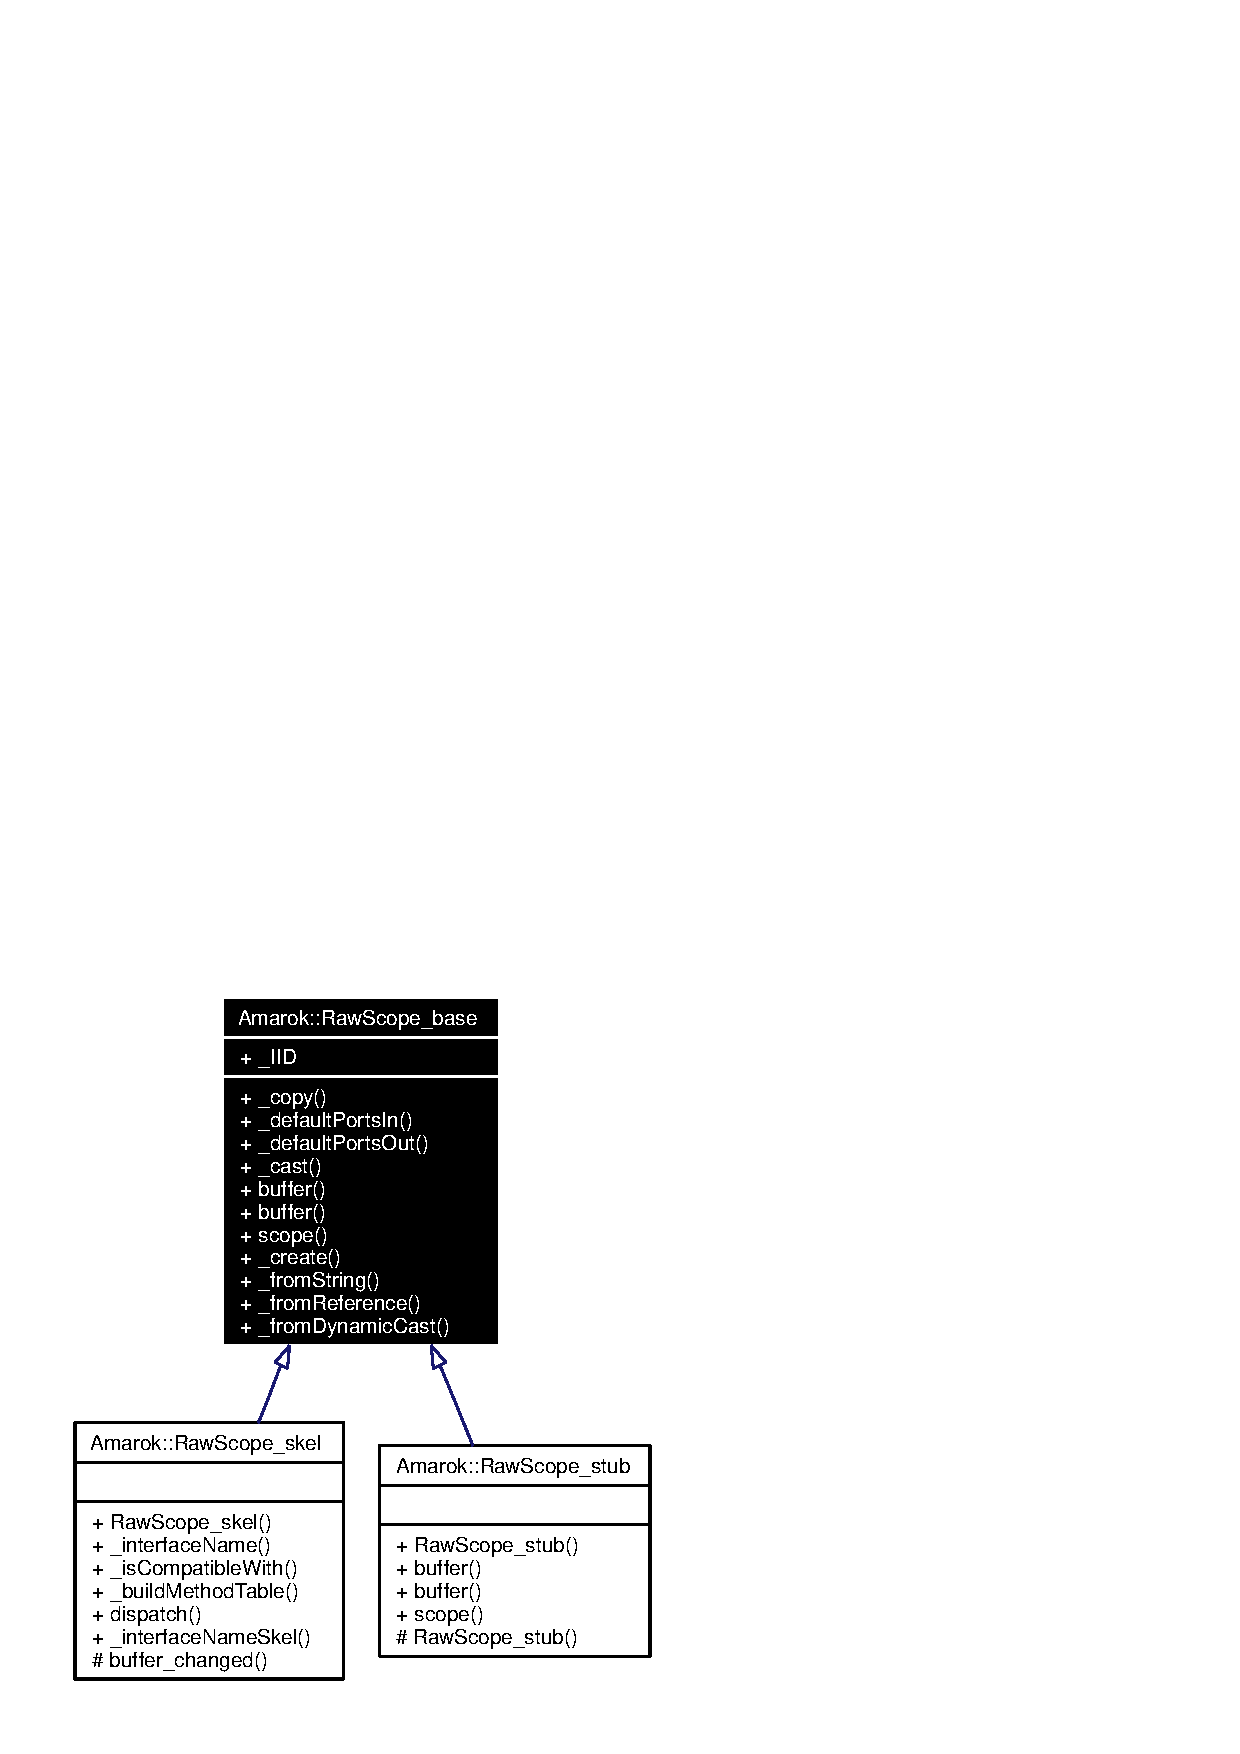
\includegraphics[width=156pt]{classAmarok_1_1RawScope__base__inherit__graph}
\end{center}
\end{figure}
\subsection*{Public Member Functions}
\begin{CompactItemize}
\item 
{\bf Raw\-Scope\_\-base} $\ast$ {\bf \_\-copy} ()
\item 
virtual std::vector$<$ std::string $>$ {\bf \_\-default\-Ports\-In} () const 
\item 
virtual std::vector$<$ std::string $>$ {\bf \_\-default\-Ports\-Out} () const 
\item 
void $\ast$ {\bf \_\-cast} (unsigned long iid)
\item 
virtual long {\bf buffer} ()=0
\item 
virtual void {\bf buffer} (long new\-Value)=0
\item 
virtual std::vector$<$ float $>$ $\ast$ {\bf scope} ()=0
\end{CompactItemize}
\subsection*{Static Public Member Functions}
\begin{CompactItemize}
\item 
{\bf Raw\-Scope\_\-base} $\ast$ {\bf \_\-create} (const std::string \&sub\-Class=\char`\"{}Amarok::Raw\-Scope\char`\"{})
\item 
{\bf Raw\-Scope\_\-base} $\ast$ {\bf \_\-from\-String} (const std::string \&objectref)
\item 
{\bf Raw\-Scope\_\-base} $\ast$ {\bf \_\-from\-Reference} (Arts::Object\-Reference ref, bool needcopy)
\item 
{\bf Raw\-Scope\_\-base} $\ast$ {\bf \_\-from\-Dynamic\-Cast} (const Arts::Object \&object)
\end{CompactItemize}
\subsection*{Static Public Attributes}
\begin{CompactItemize}
\item 
unsigned long {\bf \_\-IID} = Arts::MCOPUtils::make\-IID(\char`\"{}Amarok::Raw\-Scope\char`\"{})
\end{CompactItemize}


\subsection{Member Function Documentation}
\index{Amarok::RawScope_base@{Amarok::Raw\-Scope\_\-base}!_cast@{\_\-cast}}
\index{_cast@{\_\-cast}!Amarok::RawScope_base@{Amarok::Raw\-Scope\_\-base}}
\subsubsection{\setlength{\rightskip}{0pt plus 5cm}void $\ast$ Amarok::Raw\-Scope\_\-base::\_\-cast (unsigned long {\em iid})}\label{classAmarok_1_1RawScope__base_Amarok_1_1RawScope__stuba7}




Definition at line 249 of file amarokarts.cc.

References \_\-IID.

Referenced by \_\-from\-Dynamic\-Cast(), and Amarok::Raw\-Scope::\_\-method\_\-call().



\footnotesize\begin{verbatim}250 {
251         if(iid == Amarok::RawScope_base::_IID) return (Amarok::RawScope_base *)this;
252         if(iid == Arts::StereoEffect_base::_IID) return (Arts::StereoEffect_base *)this;
253         if(iid == Arts::SynthModule_base::_IID) return (Arts::SynthModule_base *)this;
254         if(iid == Arts::Object_base::_IID) return (Arts::Object_base *)this;
255         return 0;
256 }
\end{verbatim}\normalsize 
\index{Amarok::RawScope_base@{Amarok::Raw\-Scope\_\-base}!_copy@{\_\-copy}}
\index{_copy@{\_\-copy}!Amarok::RawScope_base@{Amarok::Raw\-Scope\_\-base}}
\subsubsection{\setlength{\rightskip}{0pt plus 5cm}{\bf Raw\-Scope\_\-base}$\ast$ Amarok::Raw\-Scope\_\-base::\_\-copy ()\hspace{0.3cm}{\tt  [inline]}}\label{classAmarok_1_1RawScope__base_Amarok_1_1RawScope__stuba4}




Definition at line 139 of file amarokarts.h.

Referenced by \_\-from\-Dynamic\-Cast().



\footnotesize\begin{verbatim}139                                       {
140                 assert(_refCnt > 0);
141                 _refCnt++;
142                 return this;
143         }
\end{verbatim}\normalsize 
\index{Amarok::RawScope_base@{Amarok::Raw\-Scope\_\-base}!_create@{\_\-create}}
\index{_create@{\_\-create}!Amarok::RawScope_base@{Amarok::Raw\-Scope\_\-base}}
\subsubsection{\setlength{\rightskip}{0pt plus 5cm}{\bf Amarok::Raw\-Scope\_\-base} $\ast$ Amarok::Raw\-Scope\_\-base::\_\-create (const std::string \& {\em sub\-Class} = \char`\"{}Amarok::Raw\-Scope\char`\"{})\hspace{0.3cm}{\tt  [static]}}\label{classAmarok_1_1RawScope__base_Amarok_1_1RawScope__stube0}




Definition at line 182 of file amarokarts.cc.

References \_\-IID.

Referenced by Amarok::Raw\-Scope::\_\-Creator().



\footnotesize\begin{verbatim}183 {
184         Arts::Object_skel *skel = Arts::ObjectManager::the()->create(subClass);
185         assert(skel);
186         Amarok::RawScope_base *castedObject = (Amarok::RawScope_base *)skel->_cast(Amarok::RawScope_base::_IID);
187         assert(castedObject);
188         return castedObject;
189 }
\end{verbatim}\normalsize 
\index{Amarok::RawScope_base@{Amarok::Raw\-Scope\_\-base}!_defaultPortsIn@{\_\-defaultPortsIn}}
\index{_defaultPortsIn@{\_\-defaultPortsIn}!Amarok::RawScope_base@{Amarok::Raw\-Scope\_\-base}}
\subsubsection{\setlength{\rightskip}{0pt plus 5cm}std::vector$<$ std::string $>$ Amarok::Raw\-Scope\_\-base::\_\-default\-Ports\-In () const\hspace{0.3cm}{\tt  [virtual]}}\label{classAmarok_1_1RawScope__base_Amarok_1_1RawScope__stuba5}




Definition at line 236 of file amarokarts.cc.



\footnotesize\begin{verbatim}236                                                                 {
237         std::vector<std::string> ret;
238         ret.push_back("inleft");
239         ret.push_back("inright");
240         return ret;
241 }
\end{verbatim}\normalsize 
\index{Amarok::RawScope_base@{Amarok::Raw\-Scope\_\-base}!_defaultPortsOut@{\_\-defaultPortsOut}}
\index{_defaultPortsOut@{\_\-defaultPortsOut}!Amarok::RawScope_base@{Amarok::Raw\-Scope\_\-base}}
\subsubsection{\setlength{\rightskip}{0pt plus 5cm}std::vector$<$ std::string $>$ Amarok::Raw\-Scope\_\-base::\_\-default\-Ports\-Out () const\hspace{0.3cm}{\tt  [virtual]}}\label{classAmarok_1_1RawScope__base_Amarok_1_1RawScope__stuba6}




Definition at line 242 of file amarokarts.cc.



\footnotesize\begin{verbatim}242                                                                  {
243         std::vector<std::string> ret;
244         ret.push_back("outleft");
245         ret.push_back("outright");
246         return ret;
247 }
\end{verbatim}\normalsize 
\index{Amarok::RawScope_base@{Amarok::Raw\-Scope\_\-base}!_fromDynamicCast@{\_\-fromDynamicCast}}
\index{_fromDynamicCast@{\_\-fromDynamicCast}!Amarok::RawScope_base@{Amarok::Raw\-Scope\_\-base}}
\subsubsection{\setlength{\rightskip}{0pt plus 5cm}{\bf Amarok::Raw\-Scope\_\-base} $\ast$ Amarok::Raw\-Scope\_\-base::\_\-from\-Dynamic\-Cast (const Arts::Object \& {\em object})\hspace{0.3cm}{\tt  [static]}}\label{classAmarok_1_1RawScope__base_Amarok_1_1RawScope__stube3}




Definition at line 200 of file amarokarts.cc.

References \_\-cast(), \_\-copy(), \_\-from\-String(), and \_\-IID.



\footnotesize\begin{verbatim}201 {
202         if(object.isNull()) return 0;
203 
204         Amarok::RawScope_base *castedObject = (Amarok::RawScope_base *)object._base()->_cast(Amarok::RawScope_base::_IID);
205         if(castedObject) return castedObject->_copy();
206 
207         return _fromString(object._toString());
208 }
\end{verbatim}\normalsize 


Here is the call graph for this function:\begin{figure}[H]
\begin{center}
\leavevmode
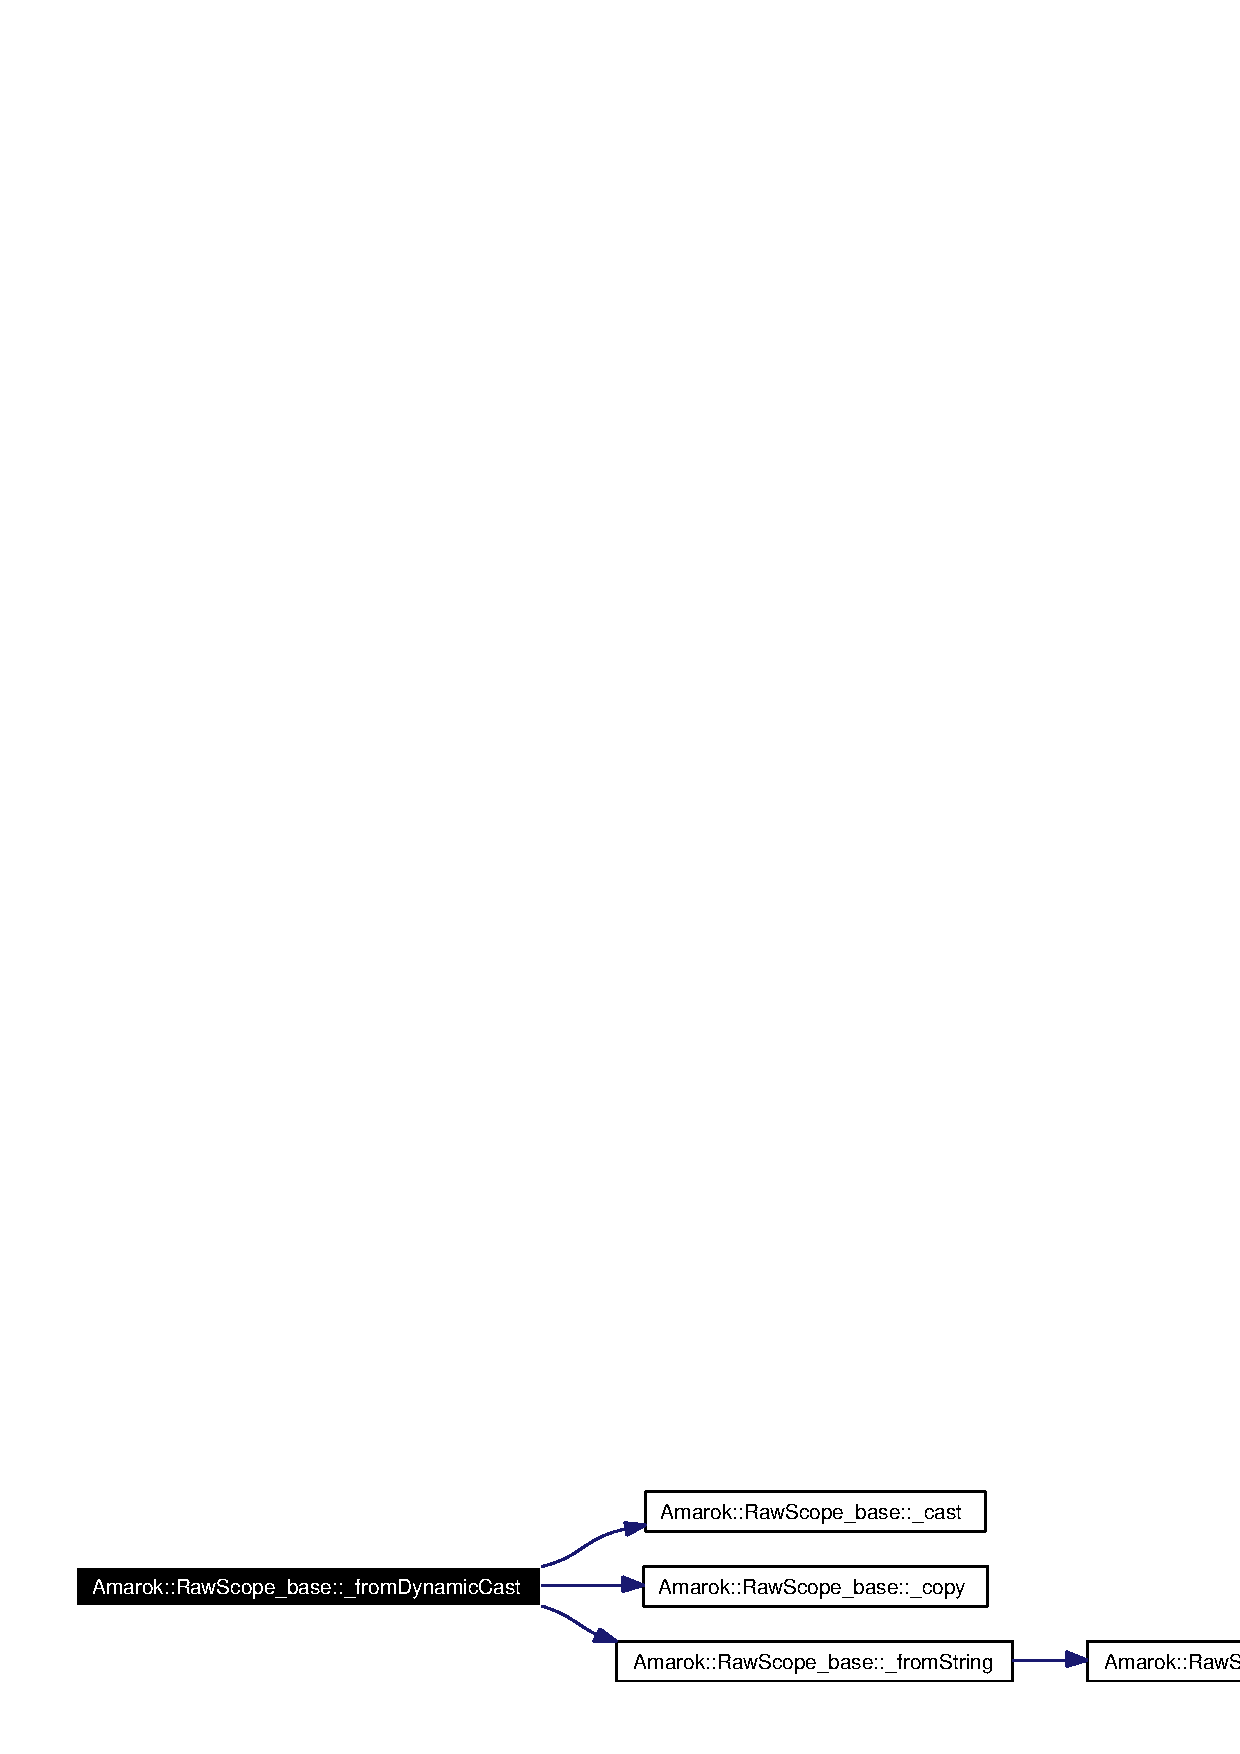
\includegraphics[width=366pt]{classAmarok_1_1RawScope__base_Amarok_1_1RawScope__stube3_cgraph}
\end{center}
\end{figure}
\index{Amarok::RawScope_base@{Amarok::Raw\-Scope\_\-base}!_fromReference@{\_\-fromReference}}
\index{_fromReference@{\_\-fromReference}!Amarok::RawScope_base@{Amarok::Raw\-Scope\_\-base}}
\subsubsection{\setlength{\rightskip}{0pt plus 5cm}{\bf Amarok::Raw\-Scope\_\-base} $\ast$ Amarok::Raw\-Scope\_\-base::\_\-from\-Reference (Arts::Object\-Reference {\em ref}, bool {\em needcopy})\hspace{0.3cm}{\tt  [static]}}\label{classAmarok_1_1RawScope__base_Amarok_1_1RawScope__stube2}




Definition at line 210 of file amarokarts.cc.

Referenced by \_\-from\-String().



\footnotesize\begin{verbatim}211 {
212         Amarok::RawScope_base *result;
213         result = (Amarok::RawScope_base *)Arts::Dispatcher::the()->connectObjectLocal(r,"Amarok::RawScope");
214         if(result)
215         {
216                 if(!needcopy)
217                         result->_cancelCopyRemote();
218         }
219         else
220         {
221                 Arts::Connection *conn = Arts::Dispatcher::the()->connectObjectRemote(r);
222                 if(conn)
223                 {
224                         result = new Amarok::RawScope_stub(conn,r.objectID);
225                         if(needcopy) result->_copyRemote();
226                         result->_useRemote();
227                         if (!result->_isCompatibleWith("Amarok::RawScope")) {
228                                 result->_release();
229                                 return 0;
230                         }
231                 }
232         }
233         return result;
234 }
\end{verbatim}\normalsize 
\index{Amarok::RawScope_base@{Amarok::Raw\-Scope\_\-base}!_fromString@{\_\-fromString}}
\index{_fromString@{\_\-fromString}!Amarok::RawScope_base@{Amarok::Raw\-Scope\_\-base}}
\subsubsection{\setlength{\rightskip}{0pt plus 5cm}{\bf Amarok::Raw\-Scope\_\-base} $\ast$ Amarok::Raw\-Scope\_\-base::\_\-from\-String (const std::string \& {\em objectref})\hspace{0.3cm}{\tt  [static]}}\label{classAmarok_1_1RawScope__base_Amarok_1_1RawScope__stube1}




Definition at line 191 of file amarokarts.cc.

References \_\-from\-Reference().

Referenced by \_\-from\-Dynamic\-Cast().



\footnotesize\begin{verbatim}192 {
193         Arts::ObjectReference r;
194 
195         if(Arts::Dispatcher::the()->stringToObjectReference(r,objectref))
196                 return Amarok::RawScope_base::_fromReference(r,true);
197         return 0;
198 }
\end{verbatim}\normalsize 


Here is the call graph for this function:\begin{figure}[H]
\begin{center}
\leavevmode
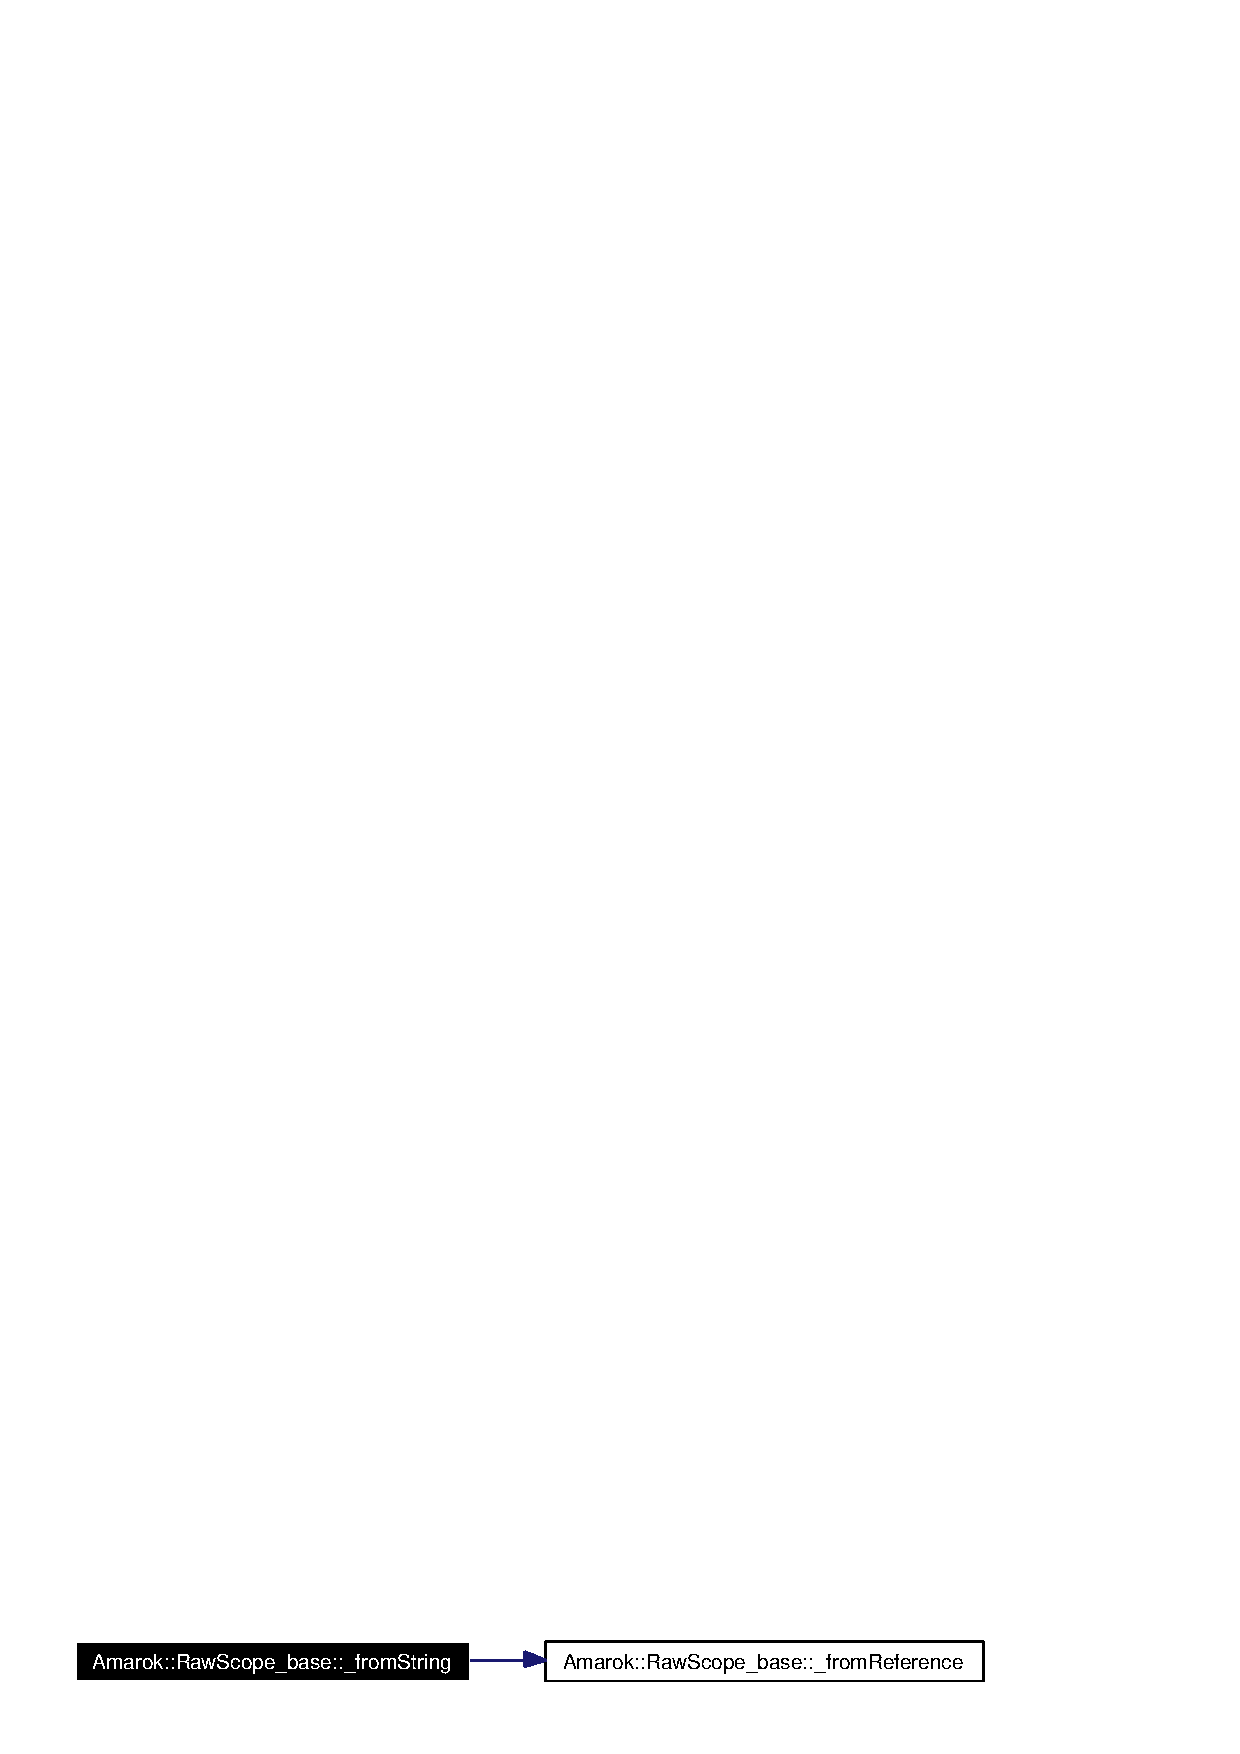
\includegraphics[width=236pt]{classAmarok_1_1RawScope__base_Amarok_1_1RawScope__stube1_cgraph}
\end{center}
\end{figure}
\index{Amarok::RawScope_base@{Amarok::Raw\-Scope\_\-base}!buffer@{buffer}}
\index{buffer@{buffer}!Amarok::RawScope_base@{Amarok::Raw\-Scope\_\-base}}
\subsubsection{\setlength{\rightskip}{0pt plus 5cm}virtual void Amarok::Raw\-Scope\_\-base::buffer (long {\em new\-Value})\hspace{0.3cm}{\tt  [pure virtual]}}\label{classAmarok_1_1RawScope__base_Amarok_1_1RawScope__skela10}




Implemented in {\bf Amarok::Raw\-Scope\_\-stub} {\rm (p.\,\pageref{classAmarok_1_1RawScope__stub_Amarok_1_1RawScope__stuba2})}.\index{Amarok::RawScope_base@{Amarok::Raw\-Scope\_\-base}!buffer@{buffer}}
\index{buffer@{buffer}!Amarok::RawScope_base@{Amarok::Raw\-Scope\_\-base}}
\subsubsection{\setlength{\rightskip}{0pt plus 5cm}virtual long Amarok::Raw\-Scope\_\-base::buffer ()\hspace{0.3cm}{\tt  [pure virtual]}}\label{classAmarok_1_1RawScope__base_Amarok_1_1RawScope__skela9}




Implemented in {\bf Amarok::Raw\-Scope\_\-stub} {\rm (p.\,\pageref{classAmarok_1_1RawScope__stub_Amarok_1_1RawScope__stuba1})}.

Referenced by Amarok::Raw\-Scope::buffer().\index{Amarok::RawScope_base@{Amarok::Raw\-Scope\_\-base}!scope@{scope}}
\index{scope@{scope}!Amarok::RawScope_base@{Amarok::Raw\-Scope\_\-base}}
\subsubsection{\setlength{\rightskip}{0pt plus 5cm}virtual std::vector$<$float$>$$\ast$ Amarok::Raw\-Scope\_\-base::scope ()\hspace{0.3cm}{\tt  [pure virtual]}}\label{classAmarok_1_1RawScope__base_Amarok_1_1RawScope__skela11}




Implemented in {\bf Amarok::Raw\-Scope\_\-stub} {\rm (p.\,\pageref{classAmarok_1_1RawScope__stub_Amarok_1_1RawScope__stuba3})}.

Referenced by Amarok::Raw\-Scope::scope().

\subsection{Member Data Documentation}
\index{Amarok::RawScope_base@{Amarok::Raw\-Scope\_\-base}!_IID@{\_\-IID}}
\index{_IID@{\_\-IID}!Amarok::RawScope_base@{Amarok::Raw\-Scope\_\-base}}
\subsubsection{\setlength{\rightskip}{0pt plus 5cm}unsigned long {\bf Amarok::Raw\-Scope\_\-base::\_\-IID} = Arts::MCOPUtils::make\-IID(\char`\"{}Amarok::Raw\-Scope\char`\"{})\hspace{0.3cm}{\tt  [static]}}\label{classAmarok_1_1RawScope__base_Amarok_1_1RawScope__stubs0}




Definition at line 381 of file amarokarts.cc.

Referenced by \_\-cast(), \_\-create(), and \_\-from\-Dynamic\-Cast().

The documentation for this class was generated from the following files:\begin{CompactItemize}
\item 
{\bf amarokarts.h}\item 
{\bf amarokarts.cc}\end{CompactItemize}
